\documentclass[plainsections, a0,  25pt]{sciposter} % 36pt no ppt eh 24pt
\usepackage[english, portuguese]{babel}
\usepackage{xcolor,eso-pic,graphicx,wallpaper}
\usepackage{fix-cm} % Huge
\usepackage{amsfonts,wrapfig} %simbolos matematicos
\usepackage{amssymb,amsmath,amsthm } %simbolos matematicos
\usepackage{textcomp}
\usepackage{psfrag, color,ifpdf,multicol,xspace}
\usepackage[utf8]{inputenc}


\usepackage[algo2e, portuguese, linesnumbered, ruled, lined, vlined, tworuled ]{algorithm2e}


\tolerance=1
\emergencystretch=\maxdimen
\hyphenpenalty=10000
\hbadness=10000

%\renewcommand{\sfdefault}{verdana}
%\usepackage{verbatim}
\usepackage{graphicx}%
\usepackage{color}
%\usepackage[small,bf]{caption}

%\usepackage{gtamacverdana}
%\usepackage{verdana}

\providecommand{\U}[1]{\protect\rule{.1in}{.1in}}
%EndMSIPreambleData
\setcounter{tocdepth}{4}

%\newenvironment{algoritmo}[1][Algoritmo:]{\noindent\textbf{#1} }{~}

\renewenvironment{proof}[1][Demonstração:]{\noindent\textbf{#1} }{\hfill   \rule{0.5em}{0.5em} \vspace{1cm}}
\newenvironment{example}[1][Exemplo]{\addtocounter{theorem}{1} \noindent\textbf{#1 \arabic{theorem}.} }{\hfill \rule{0.5em}{0.5em}  \vspace{1cm}}
\newenvironment{examples}[1][Exemplos]{\addtocounter{theorem}{1} \noindent\textbf{#1 \arabic{theorem}.} }{\hfill  \rule{0.5em}{0.5em} \vspace{1cm}}
%\newtheorem*{example}{Exemplo}
\newcounter{theorem}
\newtheorem*{acknowledgement}{Acknowledgement}
\newtheorem*{axiom}{Axiom}
\newtheorem*{case}{Case}
\newtheorem*{claim}{Claim}
\newtheorem*{conclusion}{Conclusion}
\newtheorem*{condition}{Condition}
\newtheorem*{conjecture}{Conjecture}
\newtheorem*{corollary}{Corollary}
\newtheorem*{criterion}{Criterion}
\newtheorem*{defi}{Definition}
%\newtheorem*{example}{Exemplo}
%\newtheorem*{examples}{Exemplos}
\newtheorem*{exercise}{Exercise}
\newtheorem*{lemma}{Lema}
\newtheorem*{lema}{Lema}
\newtheorem*{notation}{Notation}
\newtheorem*{problem}{Problem}
\newtheorem*{prop}{Proposition}
\newtheorem*{remark}{Remark}
\newtheorem*{solution}{Solution}
\newtheorem*{summary}{Summary}
\newtheorem*{teo}{Theorem}
\newtheorem*{obser}{Observação}

%opening
\usepackage{babel}


\definecolor{amarelo}{HTML}{FFCC00}
\definecolor{verde}{HTML}{006600}
\renewcommand{\papertype}{custom}
\setlength{\paperwidth}{90cm}
\setlength{\paperheight}{100cm}
\renewcommand{\setpspagesize}{
  \ifthenelse{\equal{\orientation}{portrait}}{
    \special{papersize=90cm,100cm}
    }{\special{papersize=90cm,100cm}
  }
}
\setlength{\topmargin}{0in}
\setlength{\headheight}{0in}
\setlength{\headsep}{0in}
\setlength{\textheight}{84cm}
\setlength{\textwidth}{80cm}%{75.5cm}
\setlength{\oddsidemargin}{0cm}%{2.4cm}
\setlength{\evensidemargin}{0cm}
\setlength{\parindent}{0in}%{0.25in}
\setlength{\parskip}{0.25in}
\setlength{\pdfpagewidth}{90cm}
\setlength{\pdfpageheight}{100cm}
\newcommand\BackgroundPic{
  \put(-82,65){
    \parbox[b][\paperheight]{\paperwidth}{%
      \vfill
      \centering
      
\includegraphics[width=\paperwidth,height=\paperheight,
      keepaspectratio]{poster-sic.jpg}%
      \vfill
    }
  }
}
\setlength{\columnseprule}{0pt}

\renewcommand{\titlesize}{\fontsize{84}{35}\selectfont }
\newcommand{\largo}{\fontsize{36}{40}\selectfont } %{36}{40}
\makeatletter
% La commande \section est définie comme suit
\renewcommand\section{\@startsection {section}{1}{\z@}%
                                   {-2ex \@plus -1ex \@minus -.1ex}%
                                   {0.8ex \@plus.1ex}%
                                   {\normalfont\largo\bfseries}}
\makeatother
\vspace{-1cm}

\def\thesection{}

%%%%%%%%%%%%%%%%%%%%%%%%%%%%%%%%%%%%%%%%%%%%%%%%%%%%%%%%%%%%%%%%%%%
%%%%%%%%%%%%%%%%%%%%%%%%%%%%%%%%%%%%%%%%%%%%%%%%%%%%%%%%%%%%%%%%%%%
%%%%%%%%%%%%%%%%%%%%%%%%%%%%   Título   %%%%%%%%%%%%%%%%%%%%%%%%%%%
\title{
  \vspace{-3cm} 
  \hspace{-25cm}
  \textcolor{amarelo}{
    \parbox{0.9\textwidth}{
      \textsc{Um sistema para auxiliar na\\ 
        aprendizagem da disciplina\\ 
        Linguagens Formais e Autômatos
      }
    }
  }
}
%%%%%%%%%%%%%%%%%%%%%%%%%%%%%%%%%%%%%%%%%%%%%%%%%%%%%%%%%%%%%%%%%%%
%%%%%%%%%%%%%%%%%%%%%%%%%%%%%%%%%%%%%%%%%%%%%%%%%%%%%%%%%%%%%%%%%%%
%%%%%%%%%%%%%%%%%%%%%%%%%%%%%%%%%%%%%%%%%%%%%%%%%%%%%%%%%%%%%%%%%%%


\begin{document}


\AddToShipoutPicture{\BackgroundPic}
\makeatletter
\AddToShipoutPicture{%
  \setlength{\@tempdimb}{.5\paperwidth}%
  \setlength{\@tempdimc}{.5\paperheight}%
  \setlength{\unitlength}{1pt}%
  \put(\strip@pt\@tempdimb,\strip@pt\@tempdimc){%
  }%
}
\makeatother
\maketitle
%\mbox{}\vspace{6cm}

\begin{center}
\textbf{\LARGE 
  Rafael Cardoso da Silva, Daniel Morgato Martin }\\
{\large
  Centro de Matemática, Computação e Cognição, Universidade Federal do ABC\\
  Av. dos Estados, 5001, Santo André, SP\\
  \textit{rafael.cardoso@aluno.ufabc.edu.br, daniel.martin@ufabc.edu.br}
}
\end{center}

\vspace{1.2cm}
\begin{multicols}{3}
% http://tex.stackexchange.com/questions/82031/how-to-write-a-title-abstract-spanning-2-columns-in-3-column-page-using-multicol
  
\paragraph{Resumo:}
Resolver exercícios é fundamental para um aluno fixar os conceitos apresentados em aula. Por outro lado, ter seus exercícios corrigidos também é muito importante, para que ele possa avaliar o seu aprendizado. Na UFABC, a disciplina de Linguagens Formais e Autômatos contempla vários exercícios que admitem infinitas respostas, o que torna a correção deles praticamente impossível, principalmente quando as turmas são grandes. O objetivo deste projeto foi a criação e implementação de um sistema para aplicação e correção automática de exercícios envolvendo autômatos finitos determinísticos. Através do estudo de métodos e algoritmos presentes na literatura, foi possível implementar o teste de equivalência entre o autômato-resposta do aluno e o autômato-gabarito previamente armazenado no banco de dados. Ao final do projeto, o sistema foi usado em caráter experimental numa turma da UFABC da disciplina de Linguagens Formais e Autômatos, afim de testar a sua qualidade. E ao final da disciplina, a nota que os alunos obtiverem ao revolver os exercícios do sistema ajudarão a compor o conceito final de cada um na disciplina.

\noindent \textbf{Palavras-chave:} autômato finito, equivalência de autômatos, minimização de autômato, programação para web.


\section{\textsc{Introdução}}

%Na disciplina MC3106 – Linguagens Formais e Autômatos – vários exercícios da parte inicial da disciplina pedem como resposta um autômato finito determinístico. Tais exercícios são particularmente trabalhosos de se corrigir porque cada um deles admite infinitas respostas corretas e, por esse motivo, sua correção se torna exaustiva para o monitor ou docente responsável.
%
%Com o intuito de agilizar essa tarefa, este projeto propõe o desenvolvimento de um sistema web que permita ao aluno inserir seu autômato-resposta por meio de uma interface intuitiva e fácil de ser utilizada e obter um \textit{feedback} quase que imediatamente, um tempo drasticamente reduzido se comparado à correção manual. 

Um \textit{autômato finito determinístico} (também chamado de AFD ou máquina de estados) consiste de um conjunto de estados não vazio $Q$, um alfabeto $\Sigma$, um estado inicial $s \in Q$, um conjunto de estados de aceitação $F \subseteq Q$ e uma função de transição $\delta \colon Q \times \Sigma \rightarrow Q$~(HOPCROFT; MOTWANI; ULLMAN, 2006).

A seguir, dois exemplos de AFDs que reconhecer a linguagem
$\{w \in \Sigma^* :  w \text{ tem número par de símbolos } \mathtt{a}\}$.

\begin{figure}
  \centering
%  \vspace{-2cm}
  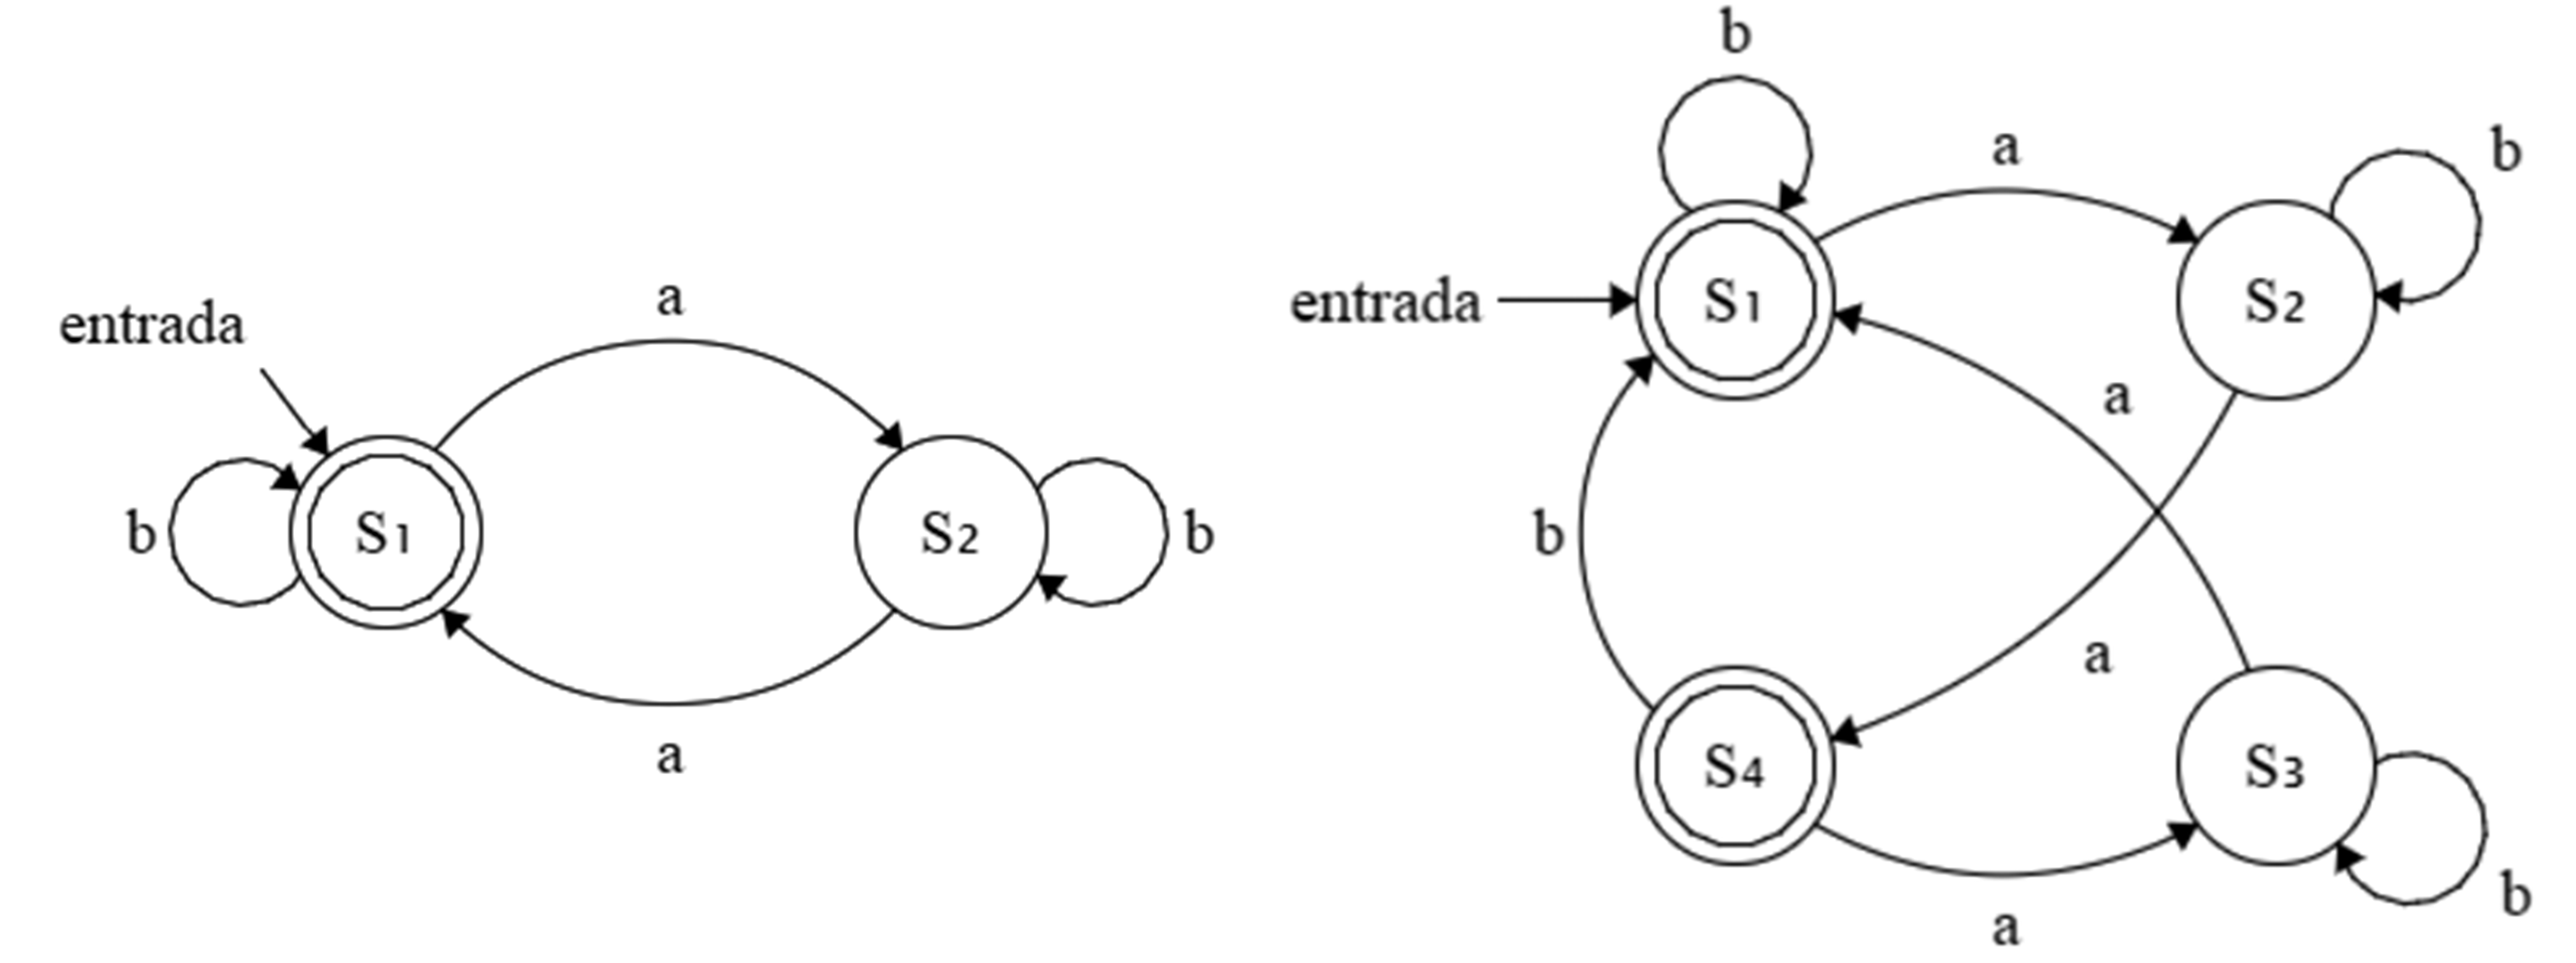
\includegraphics[width=\linewidth]{exemplo.png}
  \caption{Autômato $M_1$ a esquerda e Autômato $M_2$ a direita.}
  \label{fig:exemplo}
  \vspace{-2cm}
\end{figure}

Apesar de $M_2$ ser visivelmente maior e mais complexo que $M_1$ da Figura~\ref{fig:exemplo}, ambos reconhecem a mesma linguagem. É possível demonstrar que, para cada linguagem regular, existem infinitos autômatos que a reconhecem. Como decidir então se o autômato-resposta dado por um aluno reconhece a linguagem pedida? 

No caso do sistema que iremos desenvolver isso se reduz ao seguinte problema:
  
  
%\vspace{2cm}
{\LARGE
  \noindent\textbf{Problema:} Decidir se dois autômatos finitos determinísticos reconhecem a mesma linguagem.\par
}

%\vfill
\columnbreak



\section{\textsc{Objetivos e Metodologia}}

\begin{itemize}
\item Estudar e implementar o algoritmo de Moore para minimização e equivalência de AFDs~(MOORE, 1956);

\item Estudar e implementar o algoritmo de Hopcroft e Karp para testar a equivalência de AFDs~(HOPCROFT; KARP, 1971); 

\item Desenvolvimento do sistema de apoio a aprendizagem da disciplina Linguagens Formais e Autômatos;

\item Reuniões semanais com o orientador, afim de acompanhar o progresso do desenvolvimento do sistema e esclarecer eventuais dúvidas.
\end{itemize}



\section{\textsc{O Juiz do Sistema}}


\centerline{\textbf{Algoritmo 1:} Teste de Equivalência de Hopcroft e Karp.}
{\large
\begin{algorithm2e}[H]
    \label{alg:HKE}
    \Entrada{$ Q, \Sigma, \delta, \{p_0, q_0\}$}
    \Saida{ Conjuntos disjuntos }
    \Inicio{
      conjuntos.INIT($|Q|$) \\
      conjuntos.MERGE($p_0, q_0$) \\
      pilha.empilha($\{p_0, q_0\}$) \\
      \Enqto{pilha $\neq \emptyset$} {
        $\{p, q\} \gets$ pilha.desempilha() \\
        \ParaCada{$\sigma \in \Sigma$} {
          $r \gets$ conjuntos.FIND( $\delta(p, \sigma)$ ) \\
          $s \gets$ conjuntos.FIND( $\delta(q, \sigma)$ ) \\
          \Se{$r \neq s$} {
            conjuntos.MERGE($r, s$) \\
            pilha.empilha($\{r, s\}$) \\
          }
        }
      }
      \Retorna{conjuntos}
    }
\end{algorithm2e}

}


\section{\textsc{Modelagem do Sistema}}

\begin{figure}
  \centering
  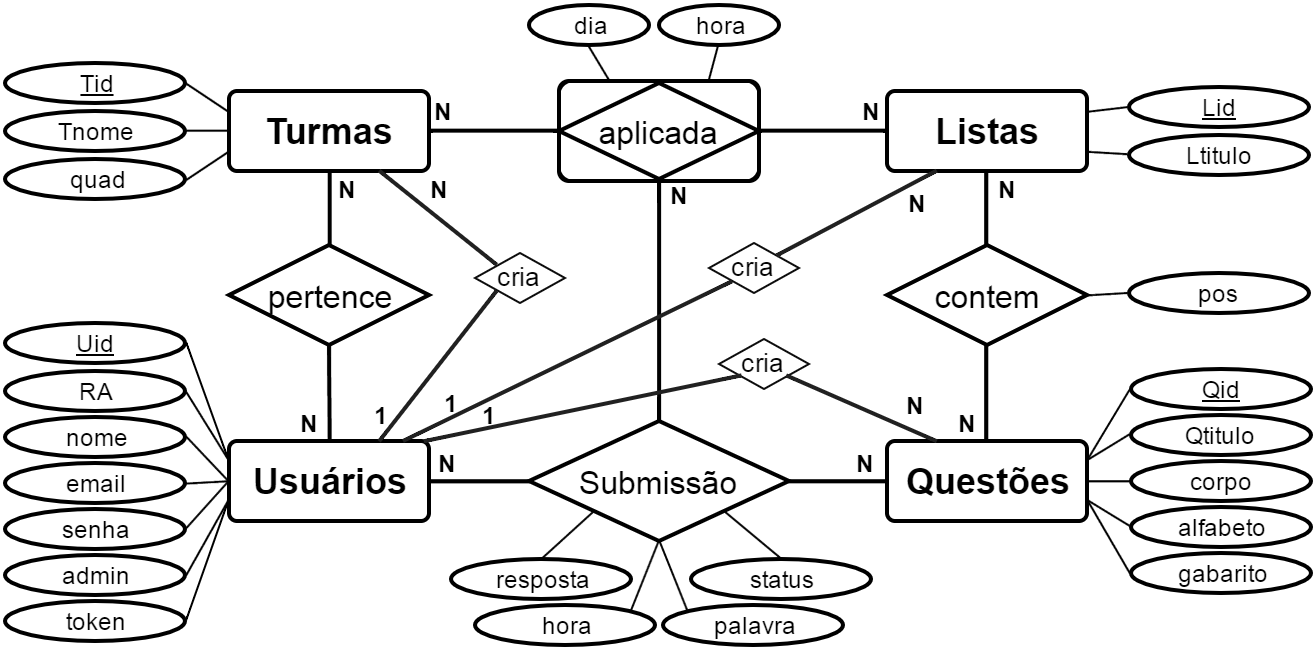
\includegraphics[width=\linewidth]{diagDER.png}
  \caption{Diagrama de Entidade e Relacionamento do DFAjudge}
  \label{fig:DER}
\end{figure}
\vspace{-1cm}

\section{\textsc{Tipos de Feedback}}
\begin{itemize}
  \item Correto;
  \item Incorreto, e uma palavra que os distinguiram;
  \item Salvo como Rascunho.
\end{itemize}


\columnbreak


\section{\textsc{Interface do DFAjudge}}

%% MAIS RESOLUCAO NO PRINT

\begin{figure}
    \vspace{-0.5cm}
  \centering
  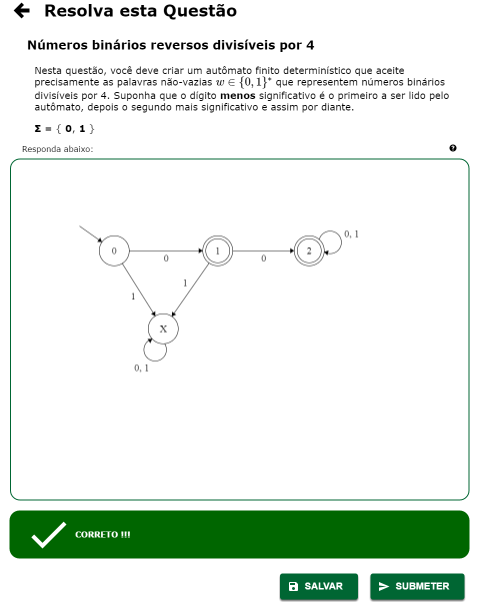
\includegraphics[width=\linewidth]{alunoResposta}
    \vspace{-0.5cm}
  \caption{Fomulário para Resolver uma Questão}
  \label{fig:alunoResposta}
  \vspace{-2cm}
\end{figure}



%\section{\textsc{Teste com a turma de 2016q2}}
%
%\begin{table}[H]
%  \centering
%  \caption{Coeficiente de correlação entre a nota obtida no sistema e nas provas.}
%  \begin{tabular}{r|r} %\hline 
%%    & Correlação \\ \hline 
%%    Porcentagem de uso do sistema e P1 & 0,443637036 \\ %\hline 
%%    Porcentagem de uso do sistema e P2 & 0,487210236 \\ %\hline 
%%    Porcentagem de uso do sistema e MP & 0,575053945 \\ %\hline 
%                      & Correlação \\ \hline 
%    Prova 1           & ~0,443637036 \\ %\hline 
%    Prova 2           & ~0,487210236 \\ %\hline 
%    Média das Provas  & ~0,575053945 \\ %\hline 
%  \end{tabular} 
%%  \vspace{-2cm}
%\end{table}


\section{\textsc{Futuros Projetos}}

\begin{itemize}
  \item Cobrir outras classes de exercícios da disciplina de Linguagens Formais e Autômatos, e também de outras disciplinas, desde que admitem algoritmos corretores;
  \item Aperfeiçoar o gerenciamento de Questões;
  \item Aprimorar o DFAdesigner;
  \item Ser aberto ao público.
\end{itemize}


\section{\textsc{Referências}}
%// apenas citados neste poster

HOPCROFT, J. E.; MOTWANI, R.; ULLMAN, J. D. \textit{Automata theory, languages, and computation}. International Edition, v. 24, 2006.

MOORE, Edward F. \textit{Gedanken-experiments on sequential machines}. Automata studies, v. 34, p. 129-153, 1956.

HOPCROFT, John E.; KARP, Richard M. \textit{A Linear Algorithm for Testing Equivalence of Finite Automata}. Technical report of Cornell University, p. 71–114, 1971.

\section{\textsc{Agradecimentos}}
Este trabalho foi financiado pelo Programa de Iniciação Científica da UFABC.


\end{multicols}
\end{document}